%%%%
% Consiglio la visione dei seguenti tutorial:
% - https://www.youtube.com/watch?v=ihxSUsJB_14
% - https://www.youtube.com/watch?v=XTFWaV55uDo
%%%%
\documentclass[12pt,a4paper,openright,twoside]{book}
\usepackage[utf8]{inputenc}

\newcommand{\thesislang}{italian} % decommentare in caso di tesi in italiano
%\newcommand{\thesislang}{english} % commentare in caso di tesi in italiano
\usepackage{thesis-style}

\begin{document}
	
\frontmatter

% ! TeX root = thesis-main.tex
\title{Title}
\author{Candidate Name Here}
\date{\today}

\begin{titlepage}
	\begin{center}
		% \vspace*{0.2cm}
		
		\large
		\textbf{ALMA MATER STUDIORUM -- UNIVERSITÀ DI BOLOGNA \\ CAMPUS DI CESENA}
		\\
		\noindent\hrulefill
		\vspace{0.4cm}
		
		\Large
		Scuola di Ingegneria e Architettura \\
		Corso di Laurea Magistrale in Ingegneria e Scienze Informatiche
		
		\Huge
		\vspace{4cm}
		\textbf{Assignment \#01}
		
		\large
		\vspace{1cm}
		Elaborato in 
		\\
		\textsc{Programmazione concorrente e distribuita}
		
		\vspace{5.5cm}
		\begin{minipage}[t]{0.64\textwidth}
			\begin{flushleft}
			\end{flushleft}
		\end{minipage}
		\begin{minipage}[t]{0.34\textwidth}
			\begin{flushright}
				\textit{Studenti} 
				\\ 
				\textbf{Eddie Barzi}
				\\ 
				\textbf{Filippo Vissani}
			\end{flushright}
		\end{minipage}\\
		
		\vfill
		\noindent\hrulefill
		\vspace{0.3cm}
		\Large

		Anno Accademico 2021-2022
	\end{center}
\end{titlepage}
\restoregeometry


%----------------------------------------------------------------------------------------
\tableofcontents   
%\listoffigures     % (optional) comment if empty
%\lstlistoflistings % (optional) comment if empty
%----------------------------------------------------------------------------------------

\mainmatter

%----------------------------------------------------------------------------------------
\chapter{\introductionname}
\label{chap:introduction}
%----------------------------------------------------------------------------------------
\section{Descrizione}
Viene fornito il codice di un programma che simula il movimento di $N$ corpi su un piano bidimensionale,
soggetti a due tipi di forze:
\begin{itemize}
	\item una forza repulsiva, per cui ogni corpo $b_{i}$ esercita su ogni altro corpo $b_{j}$ una forza in modulo pari a:
	\begin{center}
		$ F_{ij} = \frac{k_{rep} \times m_{i}}{d^2_{ij}} $
	\end{center}
	Dove $m_{i}$ è la massa del corpo $b_{i}$, $k_{rep}$ è una costante data, $d_{ij}$ è la distanza fra i due corpi.
	La direzione della forza è data dal versore $(b_{i} - b_{j})$, ovvero respingente per il corpo $b_{j}$.
	\item Una forza di attrito, per cui su ogni corpo $b_{i}$ che si muove a una velocità $v_{i}$ è esercitata una forza:
	\begin{center}
		$ FR_{i} = - k_{fri} \times v_{i} $
	\end{center}
	Che si oppone al moto, quindi in direzione opposta alla sua velocità, dove $k_{fri}$ è una costante data.
\end{itemize}
Il programma è sequenziale, non strutturato. 
L'algoritmo che definisce il comportamento del simulatore in pseudo codice è il seguente:
\newpage
\begin{lstlisting}
vt = 0;     /* virtual time */         
dt  = 0.01; /* time increment at each iteration */

loop:
	For each body b[i]:
		compute total force exerted by other bodies b[j] and friction;
		compute the instant acceleration, given the total force and mass;
		update body velocity, given the acceleration and the virtual time elapsed dt;
	Update bodies positions, given the velocity and virtual time elapsed dt;
	Check boundary collisions;
    vt = vt + dt;   
    Display current stage;

\end{lstlisting}

Alcuni aspetti rilevanti in merito al comportamento del programma e alla natura del problema:
\begin{itemize}
	\item Il calcolo delle forze al tempo $t$ avviene considerando coerentemente le posizioni dei corpi al tempo $t$. 
	\item L'aggiornamento delle posizioni può avvenire solo dopo che tutte le forze sono state calcolate (e le velocità aggiornate).
	\item Il controllo della collisione con i confini del mondo per un corpo $b_{i}$ può comportare il cambiamento della velocità e posizione del corpo.
	\item Nel programma, la visualizzazione dello stato corrente della simulazione o frame (via GUI) avviene in modo sincrono, per cui la successiva iterazione avviene solo dopo aver visualizzato lo stato della precedente.
\end{itemize}

\section{Obiettivi}
\subsection{Realizzazione di una Versione Concorrente della Simulazione}
Realizzare una versione concorrente della simulazione senza GUI, considerando un insieme iniziale $N$ di corpi
- e calcolando l'evoluzione temporale per un certo numero di passi $Nsteps$ -
con $Nsteps$ fissato come parametro. Posizione e velocità iniziali possono essere definite in modo casuale.
L'obiettivo è:
\begin{itemize}
	\item Massimizzare le performance, sfruttando tutte le capacità di calcolo del generico
	sistema di elaborazione su cui è mandato in esecuzione il programma.
	\item Organizzare il programma in modo modulare, estendibile.
\end{itemize}

Analizzare le performance del programma considerando valori di $N$ pari a 100, 1000, 5000, con $Nsteps$ pari a 1000, 10000, 50000,
calcolando lo speedup, e valutando il suo comportamento usando sia il numero ottimale teorico di thread,
sia considerando prove diverse con un numero variabile di threads per verificarne la scalabilità.
Verificare la correttezza del programma usando Java Path Finder, considerando la parte più significativa in merito, opportunamente semplificata.

\subsection{Inclusione di un'Interfaccia Grafica}
Estendere la simulazione includendo una GUI con pulsanti start/stop per lanciare/fermare la simulazione e visualizzare l'andamento,
includendo informazioni circa il tempo virtuale.
La GUI si presuppone visualizzi stati consistenti della simulazione (ma non necessariamente tutti gli stati).
%----------------------------------------------------------------------------------------
\chapter{Analisi del Problema}
\label{chap:Analisi del Problema}
%----------------------------------------------------------------------------------------
Problema dell'accesso concorrente alla stessa lista di corpi, quindi è necessario parallelizzare la computazione
sincronizzando adeguatamente i flussi di esecuzione (evitando deadlock, race contition, ecc..).
Allo stesso tempo è fondamentale che i flussi di esecuzione sfruttino al massimo il tempo per la computazione evitando
attese non necessarie.
Nel portare il programma da sequenziale a parallelo bisogna fare in modo che ad ogni iterazione
la rappresentazione della simulazione sia consistente, ovvero non ci deve essere un thread che sta
calcolando la forza repulsiva su un corpo mentre un altro thread ha già aggiornato un altro corpo con la nuova posizione.
È necessario che i thread siano allineati sulla stessa iterazione.
È fondamentale che la parallelizzazione avvenga correttamente indipendentemente dalla macchina su
cui viene eseguito il programma, ovvero il numero di thread deve essere scelto rispettando la formula
$N_{cpu} + 1$ per massimizzare le performance.
Un altro aspetto da tenere in considerazione è quello che riguarda la modularità del sistema.
È bene suddividere la parte di logica dalla parte che si occupa di orchestrare la computazione
e dalla parte che si occupa della visualizzazione. in breve: tenere ben separate la componente logica,
la componente visuale e la componente di coordinamento.

%----------------------------------------------------------------------------------------
\chapter{Descrizione dell'Architettura Proposta} % possible chapter for Projects
\label{chap:Descrizione dell'Architettura Proposta}
%----------------------------------------------------------------------------------------

\begin{figure}
	\centering
	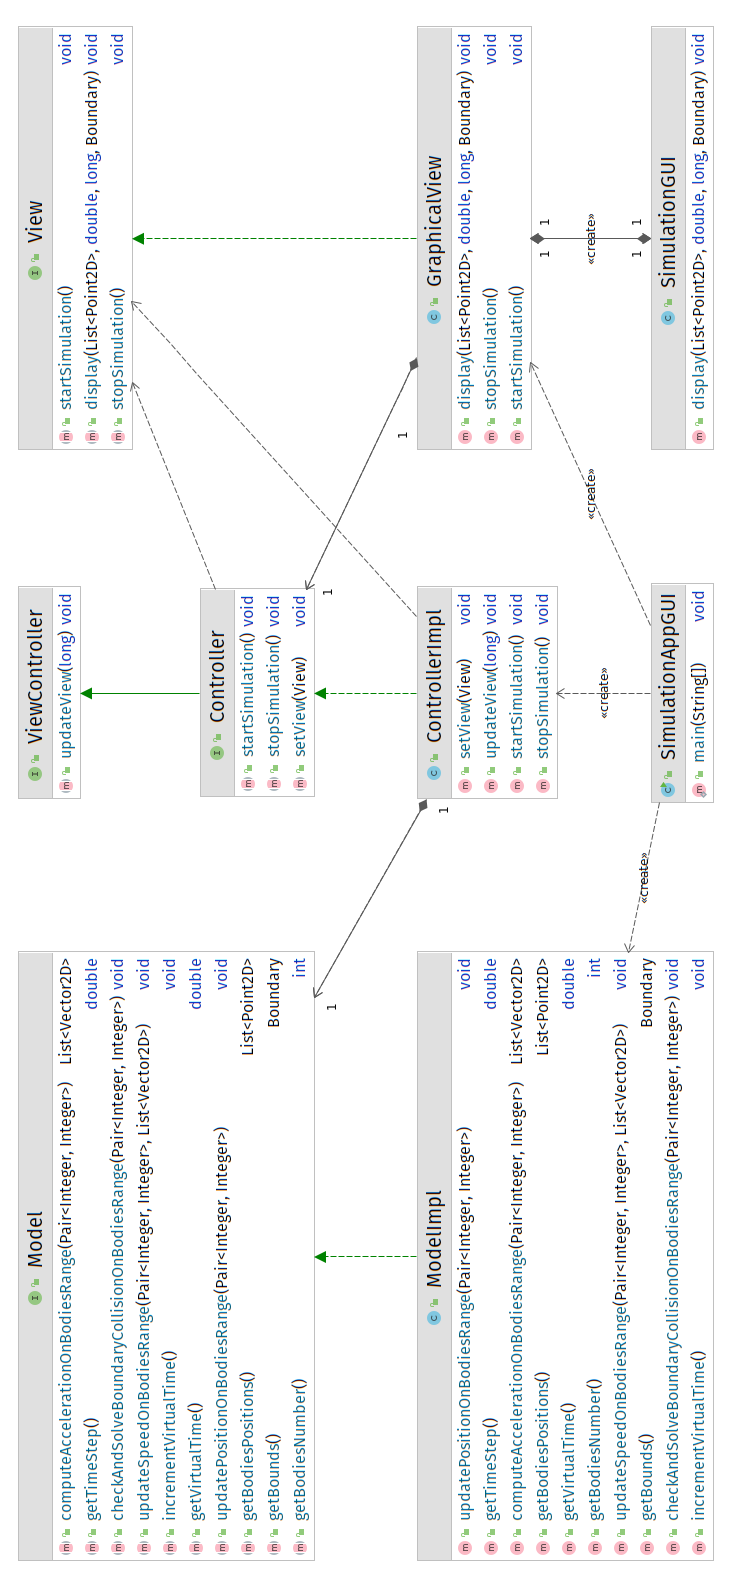
\includegraphics[width=0.7\linewidth]{figures/MVC-class-diagram.png}
	\caption{Model View Controller: diagramma delle classi.}
	\label{fig:mvc}
\end{figure}

\begin{figure}
	\centering
	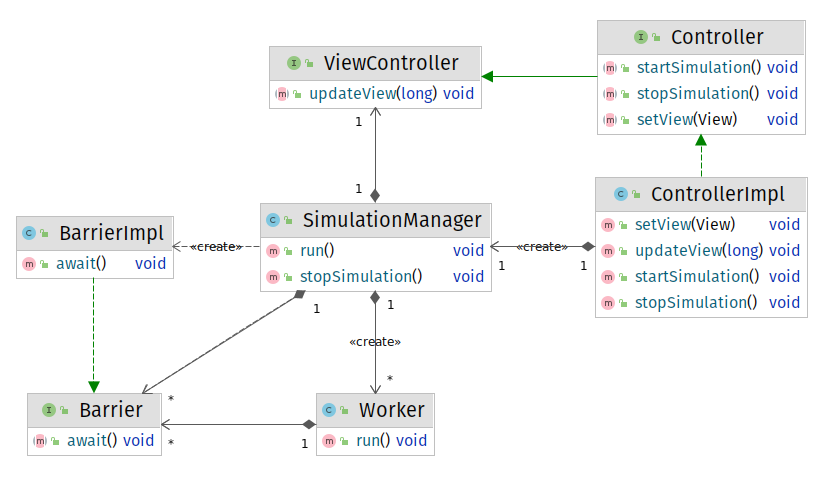
\includegraphics[width=\linewidth]{figures/simulation-manager.png}
	\caption{Simulation manager: diagramma delle classi.}
	\label{fig:SimulatioManager}
\end{figure}

%----------------------------------------------------------------------------------------
\chapter{Descrizione del Comportamento del Sistema} % possible chapter for Projects
\label{chap:Descrizione del Comportamento del Sistema}
%----------------------------------------------------------------------------------------

You may need to reference listings in your thesis.
%
In this case, you are encouraged to make them \emph{floating}, and reference them by means of labels.

%----------------------------------------------------------------------------------------
\chapter{Verifica delle Prestazioni} % possible chapter for Projects
\label{chap:Verifica delle Prestazioni}
%----------------------------------------------------------------------------------------

I test sono stati effettuati su una macchina con le seguenti caratteristiche:
\begin{itemize}
	\item Sistema operativo: Fedora 35 (GNU/Linux)
	\item Versione kernel Linux: 5.16.18
	\item Ambiente desktop: Gnome 41.5
	\item Memoria: 16GB, 3200Mhz
	\item CPU: AMD Ryzen 7 5700U
\end{itemize}
Descrizione dettagliata del processore:
\begin{itemize}
	\item Core: 8
	\item Thread: 16
	\item Clock base: 1.8GHz
	\item Clock max: 4.3GHz
	\item Cache L2: 4MB
	\item Cache L3: 8MB
\end{itemize}

Osservando i dati riportati nella tabella \ref{tab:table1}
si possono trarre le seguenti conclusioni:
\begin{itemize}
	\item Per un numero di corpi sufficientemente piccolo (in questo caso 100),
	il programma sequenziale impiega meno tempo di quello parallelo.
	\item I valori proposti relativi al numero di corpi non sono sufficienti per dimostrare che $N_{cpu}+1$
	è il numero ottimale di thread da usare. Infatti, considerando il tempo di esecuzione della simulazione con 5000 corpi e 1000 iterazioni,
	la differenza tra 9 e 17 thread è pressoché nulla
\end{itemize}

\begin{center}
	\begin{table}
		\begin{tabular}{ |c|c|c|c|c| } 
			\hline
				Corpi & Iterazioni & Thread & Tempo esecuzione (ms) & Speedup \\
			\hline
				100  & 50000  & 1 & 5612 & 1 \\
			\hline
				100  & 50000  & 9 & 13653 & 0.41 \\
			\hline
				100  & 50000  & 17 & 23923 & 0.23 \\
			\hline
				100  & 50000  & 99 & 123088 & 0.04 \\
			\hline
				1000  & 10000  & 1 & 82887 & 1 \\
			\hline
				1000  & 10000  & 9 & 40312 & 2.06 \\
			\hline
				1000  & 10000  & 17 & 44382 & 1.87 \\
			\hline
				1000  & 10000  & 99 & 46137 & 1.79 \\
			\hline
				5000  & 1000  & 1 & 183813 & 1 \\
			\hline
				5000  & 1000  & 9 & 103834 & 1.77 \\
			\hline
				5000  & 1000  & 17 & 102516 & 1.79 \\
			\hline
				5000  & 1000  & 99 & 102355 & 1.79 \\
			\hline
		\end{tabular}
		\label{tab:table1}
		\caption{Tabella con i risultati dei test}
	\end{table}
\end{center}

\begin{center}
	\begin{table}
		\begin{tabular}{ |c|c|c|c|c| } 
			\hline
				Corpi & Iterazioni & Thread & Tempo esecuzione (ms) & Speedup \\
			\hline
				50000  & 100  & 1 & ??? & 1 \\
			\hline
				50000  & 100  & 9 & ??? & ??? \\
			\hline
				50000  & 100  & 17 & ??? & ??? \\
			\hline
		\end{tabular}
		\label{tab:table2}
		\caption{Tabella con i risultati dei test}
	\end{table}
\end{center}

%----------------------------------------------------------------------------------------
\chapter{Identificazione delle Proprietà di Correttezza} % possible chapter for Projects
\label{chap:Identificazione delle Proprietà di Correttezza}
%----------------------------------------------------------------------------------------

\end{document}